\documentclass[tikz,10pt]{standalone}
\usepackage{tkz-euclide}

\definecolor{ccred}{cmyk}{0, 0.87, 0.8, 0.21}

\begin{document}
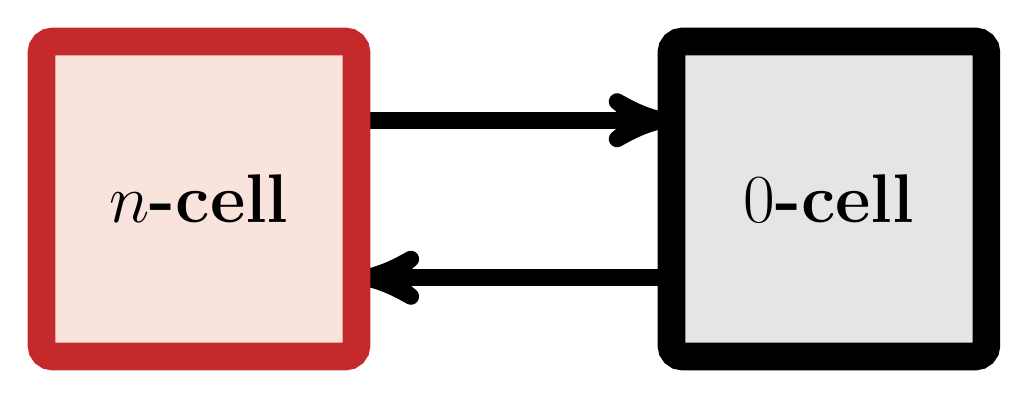
\begin{tikzpicture}[scale=2]

   % Style des flèches
  \tikzstyle{fleche} = [->, >=stealth', thick, rounded corners=4pt]
  \tikzstyle{doublefleche} = [<->, >=stealth', thick, rounded corners=4pt, line width=2]

    % n-cell <-> 0-cell
  %\draw[fleche, line width=6, black] (2,1) -- (4,1) ;
  \draw[fleche, line width=6, black] (2,1.5) -- (4,1.5) ;
  \draw[fleche, line width=6, black] (4,0.5) -- (2,0.5) ;

  % Liste des boxes
  \draw[line width=10, ccred, rounded corners, fill=ccred!10!white] (0,0) -- (2,0) -- (2,2) -- (0,2) -- cycle ;
  \draw[line width=10, black, rounded corners, fill=black!10!white] (4,0) -- (6,0) -- (6,2) -- (4,2) -- cycle ;


  \draw (1,1) node (region) {\Huge \textbf{$n$-cell}};
  \draw (5,1) node (arete) {\Huge \textbf{$0$-cell}};


\end{tikzpicture}
\end{document}